\documentclass[12pt]{article}

\usepackage{sectsty}
\usepackage{fullpage}
\usepackage{graphicx}

\sectionfont{\large}
\begin{document}\vspace{0.5in}
\begin{center}\begin{large}\textbf{Gopineedi Harsha Vardhan}\end{large}\end{center}\textbf{\hrulefill}\\

\begin{tabular}{@{}p{4in}p{3in}}
Room No-A63 & {Phone:}+91-8181939314 \\
Dr. S RadhaKrishnan Hostel & {E-mail:}harsha.gopineedi@gmail.com\\
University of Allahabad \\
Allahabad\\
& 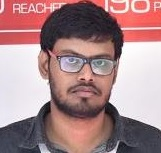
\includegraphics[scale=0.8]{harsha.jpg}\\
\end{tabular}

\section*{Objective}
To utilize my technical skills towards developing systems that are smarter and can learn by itself; providing its users experience like never before.   
\section*{Education}
\begin{tabular}{|l|l|l|l|l|}
\hline
Degree & College/School & University & Passing Year & Pass Percentage\\
\hline
B. Tech & JKIAPT & Allahabad University & 2017 & 67.8(till 5th sem)\\
\hline
Intermediate & Delhi Public School & CBSE & 2013 & 91\\
\hline
High School & Gowtham Concept School & SSC & 2011 & 90.1\\
\hline
\end{tabular}

\section*{Projects}
\begin{itemize}
\item[$\bullet$]\textbf{Puzzle Solver Robot.}\\November 2015- Feb 2016\\Members: Raj Krishna,Keshav Bihani, Shantam Srivastava

This project was based on OpenCv and Python and implemented on Atmega 2560. It used basic image processing technique to sense an image and then solve the puzzle using the input image.
\item[$\bullet$]\textbf{Face Recognition System}\\Dec 2015- Jan 2016\\

This project was based on OpenCv and Python for taking live feed from a camera and identify the person and grant acess
\item[$\bullet$]\textbf{Waste Segregating Robot.}\\October 2014-Jan 2015 \\Members: Raj Krishna,Keshav Bihani, Shantam Srivastava

This project was based on Atmega 2560 to segregate waste based on its size and colour.It did win the second position in eYRC competition amongst 52 other teams that participated.
\end{itemize}
\section*{Training and Internships}
\begin{enumerate}
\item Linux System Administration.\\May 2014- July 2014. Rroot Shell Technologies, Hyderabad.
\item Networking.\\May 2015-July 2015.Rroot Shell Technologies,Hyderabad.
\end{enumerate}
\section*{Technical Skills}
\begin{itemize}
\item[$\cdot$]Programming Languages
\begin{enumerate}
\item C
\item Java
\item Python
\end{enumerate}
\item[$\cdot$]Knowledge of Data Structures and Algorithms.
\item[$\cdot$]Tools and Technologies Used
\begin{enumerate}
\item Atmel Studio
\item Android Studio
\item OpenCV.
\end{enumerate}
\item[$\cdot$]Operating Systems
\begin{enumerate}
\item Microsoft WindowsXP and onwards
\item Red Hat Enterprise Linux 6.0 and onwards
\item Ubuntu and Fedora
\end{enumerate}
\end{itemize}
\begin{itemize}
\item[$\cdot$]
\end{itemize}
\section*{Soft Skills}
\begin{itemize}
\item[$\cdot$] Good Communication Skills with bilingual proficiency in English and Telugu.Can Also Speak and understand Hindi.
\item[$\cdot$]Flexible/Adaptable.
\item[$\cdot$]Positive Attitude.
\item[$\cdot$]Good presentation and management skills.
\end{itemize}
\section*{Extra-Curricular Activities}
\begin{itemize}
\item[$\cdot$]Robotics Competition.
\item[$\cdot$]Networking
\item[$\cdot$]Ethical Hacking
\end{itemize}
\section*{Co-Curricular Activities}
\begin{itemize}
\item[$\cdot$] Music
\item[$\cdot$] Playing Computer Games 
\item[$\cdot$] Dancing
\end{itemize}
\section*{Personal Details}
\begin{itemize}
\item[$\cdot$]Father's Name : Mr.Gopineedi Swamiji.
\item[$\cdot$]Mother's Name : Mrs.Gopineedi Bhuvaneshwari.
\item[$\cdot$]Sex           : Male.
\item[$\cdot$]Date of Birth : Sep 8,1996.
\item[$\cdot$]Nationality   : Indian.
\item[$\cdot$]Martial Status: Single.
\end{itemize}
\section*{Declaration} I hereby declare that the above information is true and authentic to the best of my knowledge.
\section*{Date} May 24,2016.

\end{document}